\section{Resultados}

Os programas foram compilados e executados de modo automatizado por \emph{shell scripts} no computador de um dos integrantes do grupo do trabalho. Seguem as especificações:

\begin{verbatim}Phoronix Test Suite v5.2.1
System Information

Hardware:
Processor: Intel Core i7-3612QM @ 3.10GHz (8 Cores),
Motherboard: Dell 0DNMM8, Chipset: Intel 3rd Gen Core DRAM, Memory: 8192MB,
Graphics: Intel HD 4000 2048MB (1100MHz)

Software:
OS: Fedora 20, Kernel: 3.15.10-201.fc20.x86_64 (x86_64),
Compiler: GCC 4.8.3 20140624, File-System: ext4
\end{verbatim}

Os resultados de tempos a seguir são provenientes de 10 execuções consecutivas dos programas no computador citado acima. Foi considerado para os testes o \texttt{input08} que acompanha a especificação do trabalho. Os arquivos completos dos resultados aqui apresentados podem ser consultados no diretório \texttt{./test} deste trabalho.

\newpage
\subsection{Floyd-Warshall}

Comparando os resultados obtidos nas execuções do programa Floyd-Warshall, pode-se constatar que a paralelização foi eficiente e as execuções ficaram cada vez mais rápidas de acordo com a quantidade de \textit{threads}, alcançando um \textit{speed up} de até $2.60$. Percebe-se também que o \textit{speed up} tende a se estabilizar conforme a quantidade de \textit{threads} aumenta, pois o sistema operacional gasta cada mais tempo com o gerenciamento das \textit{threads}.

Analisando-se o algoritmo sequencial, é possível notar que sua complexidade é $O(n^3)$, pois o maior processamento encontra-se nos 3 laços aninhados que iteram com relação à quantidade total $n$ de vértices.

\begin{table}[h]
\begin{center}
	\begin{tabular}{|c||c|c|c|c|c|} 
		\hline
		Threads & FWS & FWP & Stddev & ConfInt &\textit{Speedup} \\
		\hline

		1  & 6.827 & ---   & 0.040012 & [ 6.802200, 6.851800 ] & ---  \\
		2  & ---   & 5.647 & 0.585219 & [ 5.284278, 6.009722 ] & 1.21 \\
		4  & ---   & 4.591 & 0.609778 & [ 4.213056, 4.968944 ] & 1.49 \\
		8  & ---   & 3.289 & 0.448206 & [ 3.011199, 3.566801 ] & 2.08 \\
		16 & ---   & 2.727 & 0.372345 & [ 2.496218, 2.957782 ] & 2.50 \\
		32 & ---   & 2.628 & 0.310895 & [ 2.435305, 2.820695 ] & 2.60 \\
		
		\hline
	\end{tabular}
	\caption{Médias dos tempos (s) de 10 execuções do algoritmo Floyd-Warshall e \emph{speed-up}}
	\caption*{
		FWS: Floyd-Warshall Sequencial / FWP: Floyd-Warshall Paralelo\\
		Stddev: Desvio padrão / ConfInt: Intervalo de Confiança\\
	}
\end{center}
\end{table}

\begin{figure}[h]
\centering
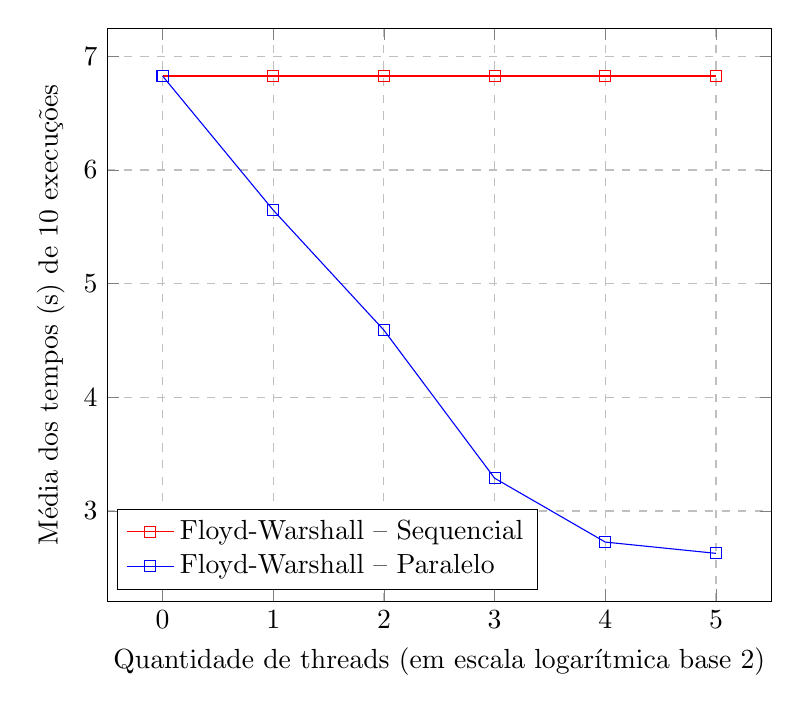
\begin{tikzpicture}
\begin{axis}[
	ylabel={Média dos tempos (s) de 10 execuções},
	xlabel={Quantidade de threads (em escala logarítmica base 2)},
	legend style={at={(0.015,0.02)},anchor=south west, legend cell align=left},
	ymajorgrids=true,
	xmajorgrids=true,
	grid style=dashed,
	/pgf/number format/1000 sep={},
	scale only axis,
	xtick = {0,1,2,3,4,5}
]
\addplot[color=red,mark=square]
coordinates{
	(0, 6.827)
	(1, 6.827)
	(2, 6.827)
	(3, 6.827)
	(4, 6.827)
	(5, 6.827)
};
\addlegendentry{Floyd-Warshall -- Sequencial}

\addplot[color=blue,mark=square]
coordinates{
	(0, 6.827)
	(1, 5.647)
	(2, 4.591)
	(3, 3.289)
	(4, 2.727)
	(5, 2.628)
};
\addlegendentry{Floyd-Warshall -- Paralelo}

\end{axis}
\end{tikzpicture}
\caption{Comparativo das médias de execução do Floyd-Warshall sequencial e paralelo}
\end{figure}

\newpage
\subsection{Dijkstra}

As estruturas de dados utilizadas na implementação do Dijkstra (listas de adjacências), implicaram em uma performace inferior em comparação à implementação com Floyd-Warshall (matriz de adjacências) apesar de possuirem uma mesma complexidade. Porém com relação ao \textit{speed up} da paralelização, obteve-se uma maior aceleração nos tempos de execução do Dijkstra como pode ser observado nos resultados. Percebe-se também uma tendência a piorar o \textit{speed up} com um número de \textit{threads} muito grande.

\begin{table}[h]
\begin{center}
	\begin{tabular}{|c||c|c|c|c|c|} 
		\hline
		Threads & DS & DP & Stddev & ConfInt &\textit{Speedup} \\
		\hline

		1  & 38.359 & ---    & 1.050176 & [ 37.708094, 39.009906 ] & ---  \\
		2  & ---    & 20.101 & 0.578921 & [ 19.742181, 20.459819 ] & 1.91 \\
		4  & ---    & 12.072 & 0.072774 & [ 12.026894, 12.117106 ] & 3.18 \\
		8  & ---    &  8.462 & 0.127891 & [  8.382733,  8.541267 ] & 4.53 \\
		16 & ---    &  8.667 & 0.515811 & [  8.347297,  8.986703 ] & 4.43 \\
		32 & ---    &  9.255 & 0.503632 & [  8.942846,  9.567154 ] & 4.14 \\
		
		\hline
	\end{tabular}
	\caption{Médias dos tempos (s) de 10 execuções do algoritmo Dijkstra e \emph{speed-up}}
	\caption*{
		DS: Dijkstra Sequencial / DP: Dijkstra Paralelo\\
		Stddev: Desvio padrão / ConfInt: Intervalo de Confiança\\
	}
\end{center}
\end{table}

\begin{figure}[h]
\centering
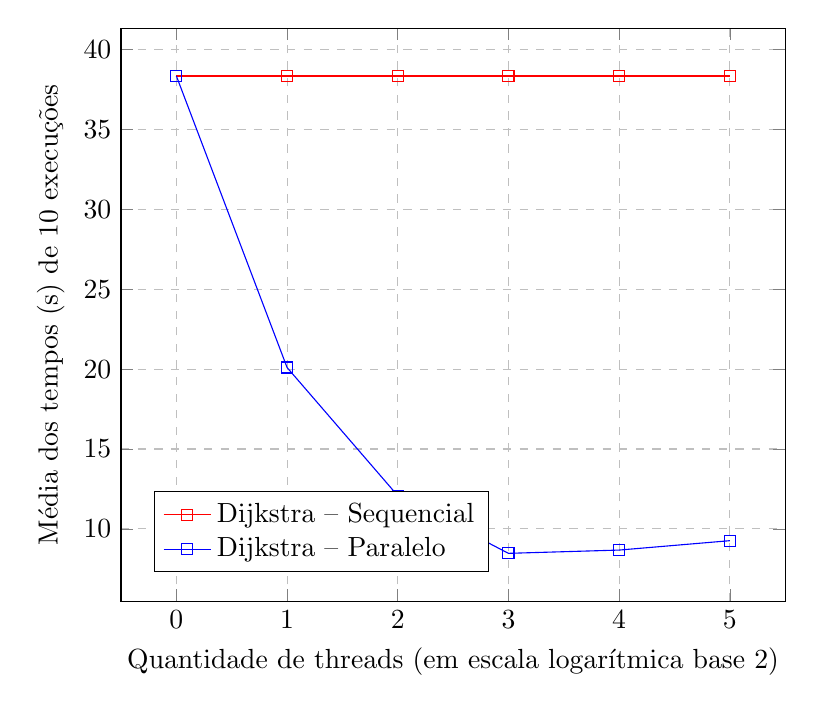
\begin{tikzpicture}
\begin{axis}[
	ylabel={Média dos tempos (s) de 10 execuções},
	xlabel={Quantidade de threads (em escala logarítmica base 2)},
	legend style={at={(0.05,0.05)},anchor=south west, legend cell align=left},
	ymajorgrids=true,
	xmajorgrids=true,
	grid style=dashed,
	/pgf/number format/1000 sep={},
	scale only axis,
	xtick = {0,1,2,3,4,5}
]
\addplot[color=red,mark=square]
coordinates{
	(0, 38.359)
	(1, 38.359)
	(2, 38.359)
	(3, 38.359)
	(4, 38.359)
	(5, 38.359)
};
\addlegendentry{Dijkstra -- Sequencial}

\addplot[color=blue,mark=square]
coordinates{
	(0, 38.359)
	(1, 20.101)
	(2, 12.072)
	(3,  8.462)
	(4,  8.667)
	(5,  9.255)
};
\addlegendentry{Dijkstra -- Paralelo}

\end{axis}
\end{tikzpicture}
\caption{Comparativo das médias de execução do Dijkstra sequencial e paralelo}
\end{figure}

